x\documentclass[10pt]{beamer}

\usepackage[utf8]{inputenc}
\usepackage{amsmath, amssymb, bm}
\usepackage{graphicx}
\usepackage{booktabs}
\usepackage{array}
\usepackage{tikz}
\usepackage{appendixnumberbeamer}
\usetikzlibrary{positioning,arrows.meta,shapes.geometric}
\usepackage[    style=authoryear,
    backend=biber,
    natbib=true,
    sorting=nyt,
    labelnumber=true]{biblatex}
\usepackage{booktabs}

\usepackage{indentfirst}
\addbibresource{reference.bib}
\usetheme{Madrid}
\usecolortheme{default}
\setbeamertemplate{navigation symbols}{}
\setbeamertemplate{footline}[frame number]

\title[Zoning and Transportation]{Zoning, Transportation Investment,\\ and Urban Sprawl}
\subtitle{Research Proposal Presentation}
\author{Ke Jiang}
\institute{Southern Methodist University}
\date{April 2026}

\newcommand{\ubar}[1]{\underline{#1}}

\begin{document}

\begin{frame}
  \titlepage
\end{frame}


\begin{frame}{Motivation}
\begin{columns}[T]
\column{0.5\textwidth}
\textbf{Zoning and city structure}
\begin{itemize}
    \item Restrictive zoning limits housing supply in desirable area,and forms job-housing separation.
    \item Households may be pushed toward cheaper but more distant locations.
    \item This raises commuting costs and sprawing development.
\end{itemize}

\column{0.5\textwidth}

\textbf{Transportation and city structure}
\begin{itemize}
    \item Rail transit can concentrate development around connected corridors and stations.
    \item Highway expansion often facilitates decentralization and suburbanization.
\end{itemize}
\end{columns}

\vspace{0.4cm}
\begin{alertblock}{Key idea}
The effect of transportation infrastructure depends on whether land around accessible locations is allowed to densify.
\end{alertblock}
\end{frame}

\begin{frame}{Research Question}
\begin{itemize}
    \item Restrictive zoning encourage sprawling development
    \item economic return to public transit is lower in low-density city\citep{Severen2021-oi}, investment turns towards roadways.
    \item Lack of public transit cause lower density development
        \item self-reinforcing...
\end{itemize}

\vspace{0.4cm}
\begin{block}{Central Question}
Does the zoning restriction actually have a larger impact if considering its effect on endogeneous public transit investment decisions?
\end{block}
\end{frame}

\begin{frame}{Research Question}
\textbf{For policymakers}:

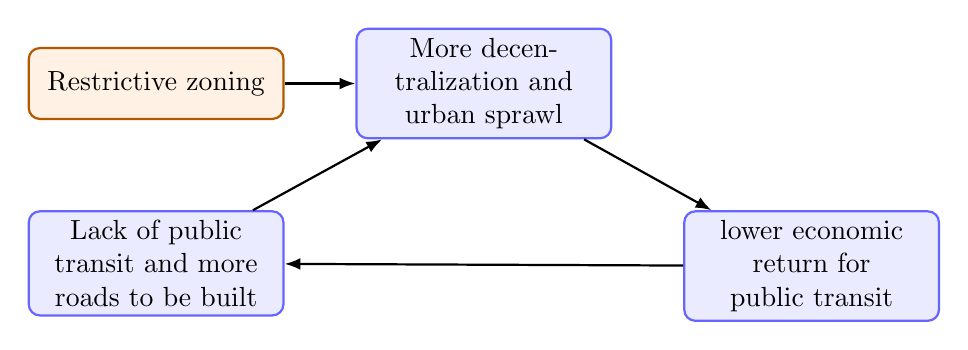
\begin{tikzpicture}[
node distance=0.9cm and 0.9cm,
box/.style={rectangle, rounded corners, draw=blue!60, fill=blue!8, thick, align=center, minimum height=0.9cm, text width=3cm},
arrow/.style={-{Latex[length=2mm]}, thick}
]

\node[box, fill=orange!10, draw=orange!70!black] (zoning) {Restrictive zoning};
\node[box, right=of zoning] (sprawl) {More decentralization and urban sprawl};
\node[box, below right=of sprawl] (invest) {lower economic return for public transit};

\node[box, below left=of sprawl] (roads) {Lack of public transit and more roads to be built};


\draw[arrow] (zoning) -- (sprawl);
\draw[arrow] (sprawl) -- (invest);
\draw[arrow] (invest) -- (roads);
\draw[arrow] (roads) -- (sprawl);

\end{tikzpicture}
\end{frame}

\begin{frame}{Relation to the Literature}
\begin{itemize}
    \item \textbf{Zoning and housing supply:} \textcite{Glaeser2003-sr},\textcite{Hsieh2019-rx}\textcite{Baum-Snow2024-ii},\textcite{Rollet2025-mk},\textcite{Glaeser2002-vq},\textcite{Bordeu2026-df},\textcite{Kashner2025-iv}

    \item \textbf{Transportation and congestion externality}:\textcite{Severen2021-oi},\textcite{Allen2025-gj},\textcite{Baum-Snow2007-zj}\textcite{Fajgelbaum2023-dr}
    \item \textbf{Urban sprawl}:\textcite{Brueckner2000-vd},\textcite{Glaeser2003-sr},\textcite{Coeurdacier2022-ip}
\end{itemize}
\
\begin{block}{Main Contribution}
\begin{enumerate}
    \item I want to show that the cost and benefit of public transit investment is in fact not exogenous but endogeneous to zoning regulations.
    \item How much is the welfare loss by comparing the counterfactual where the zoning regulation is endogenized.
\end{enumerate}
\end{block}
\end{frame}


\begin{frame}{Empirical facts(ongoing)}
\begin{block}{Planned works}
\begin{enumerate}
    \item Transportation investment decisions are driven by the economic returns (cost and benefits) 
    \item "Old" cities with developed metros before car-dominance have high returns and more transit, wheras "new" cities are oppsite
    \item Zoning laws leads to lower return to transit investment.
\end{enumerate}
\end{block}

\vspace{0.4cm}
Data source:
\begin{itemize}
    \item  National Transit Database(NTD),Transit Explore Database::"Transit volumnes, revenues and investment, operating date"
    \item Zoning: housing supply elasticity from \textcite{Baum-Snow2024-ii}
\end{itemize}
\end{frame}



\begin{frame}{Some Facts}

\begin{columns}
    
    \column{0.5\textwidth}
    \centering
    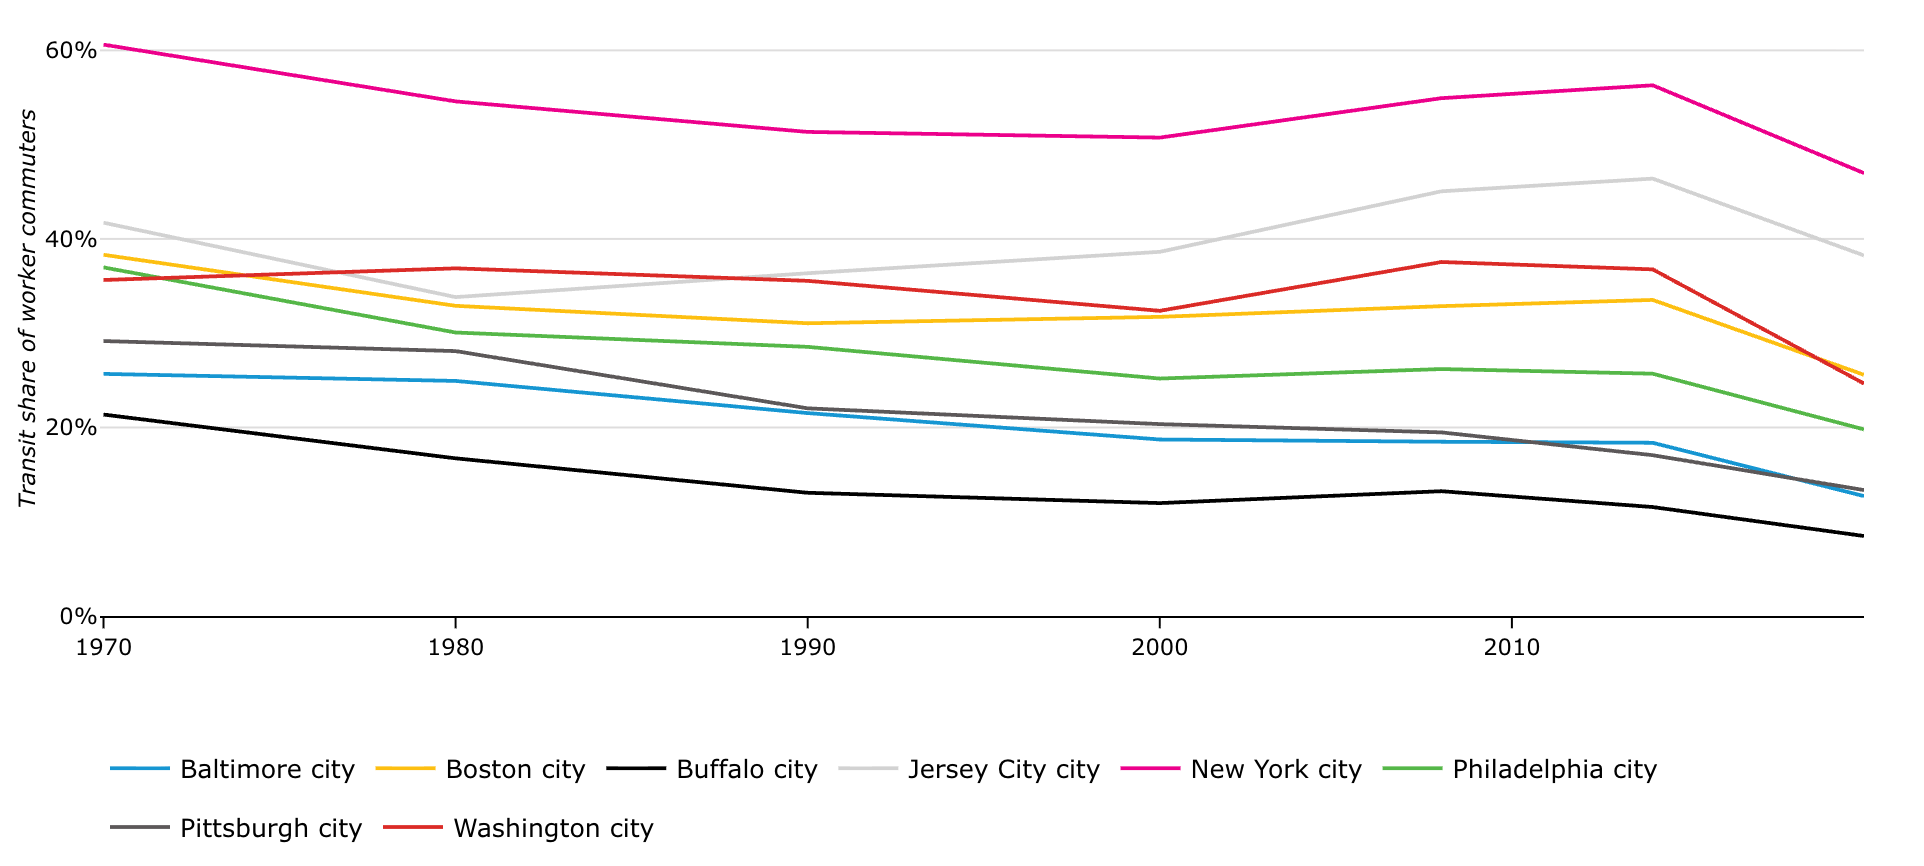
\includegraphics[width=\linewidth]{Northeast city.png}
    \\ {\footnotesize Northeast}
    
    \vspace{0.3cm}
    
    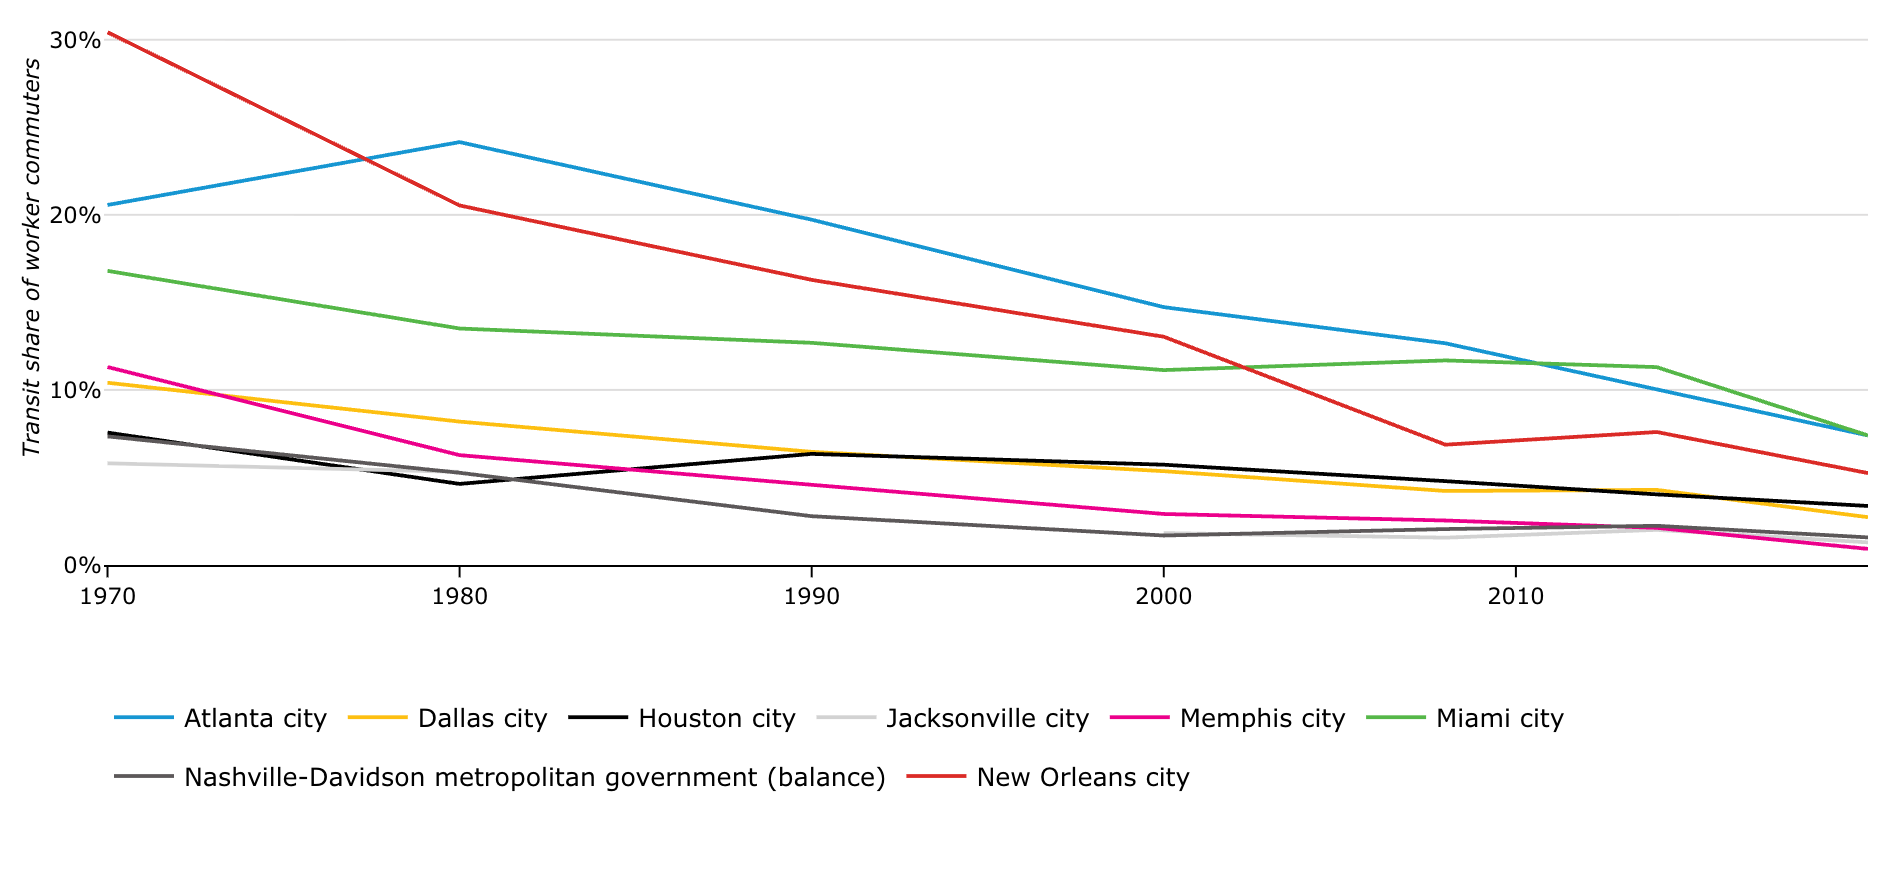
\includegraphics[width=\linewidth]{Southeast.png}
    \\ {\footnotesize Southeast}

    \column{0.5\textwidth}
    \centering
    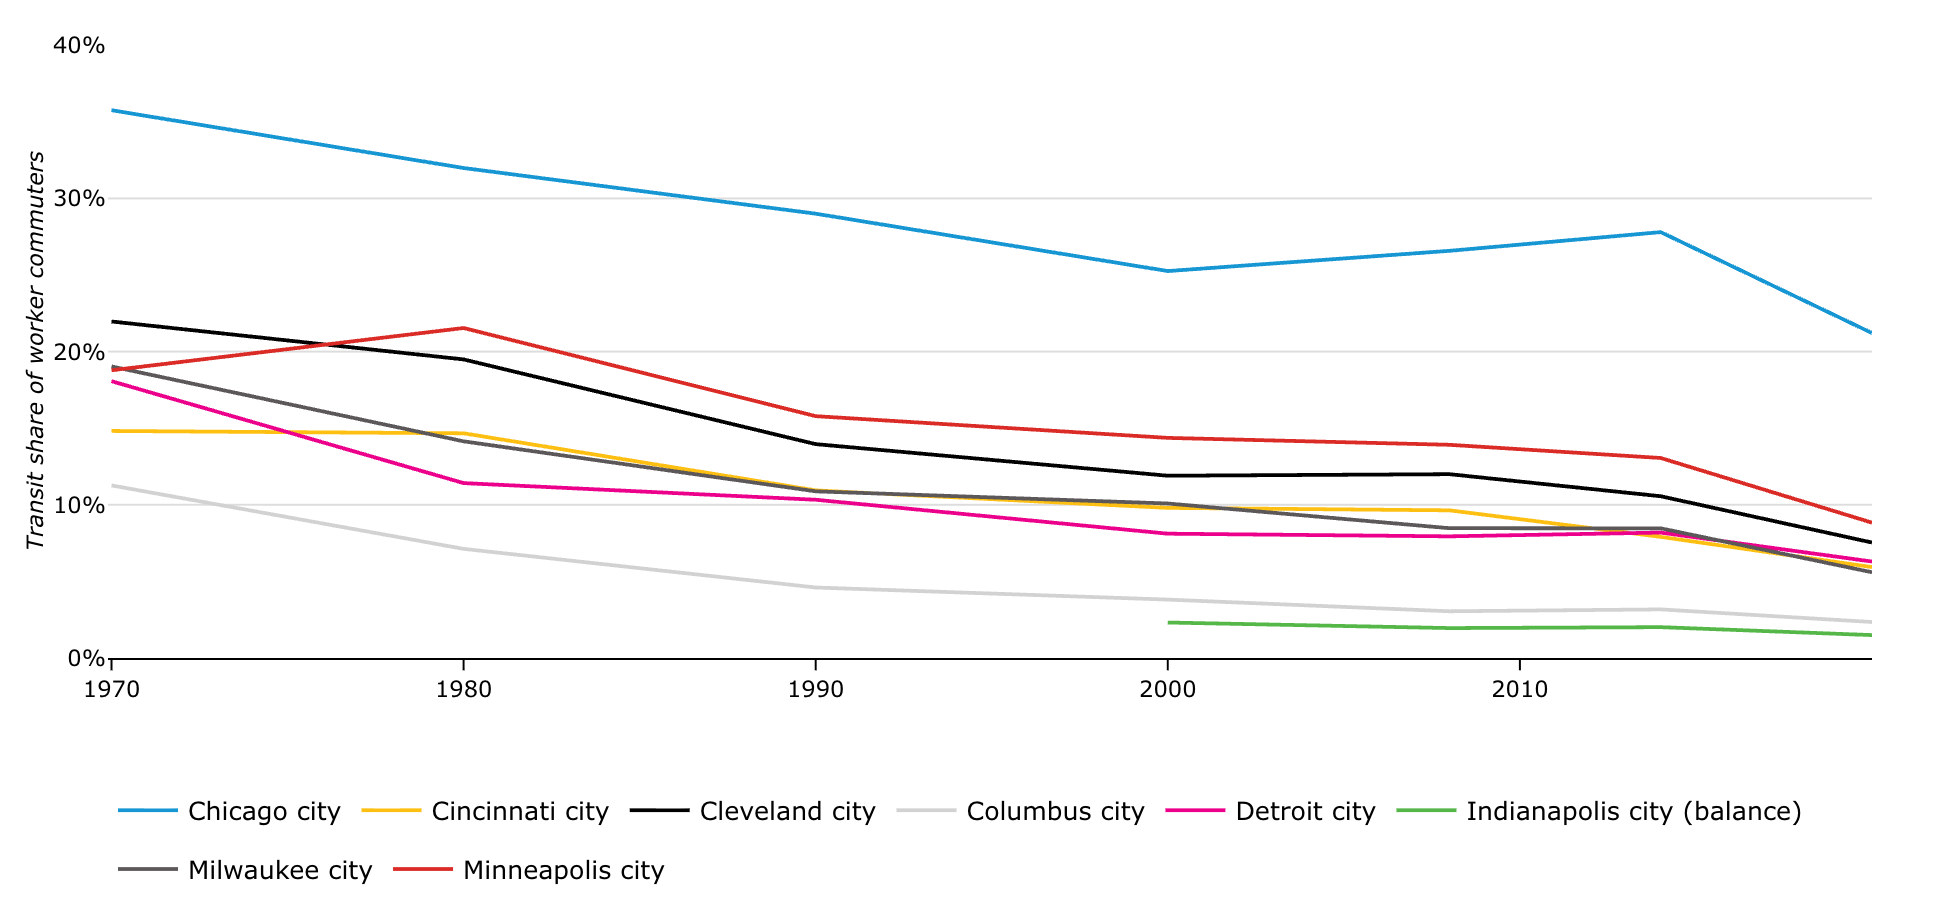
\includegraphics[width=\linewidth]{Middlewest.png}
    \\ {\footnotesize Midwest}
    
    \vspace{0.3cm}
    
    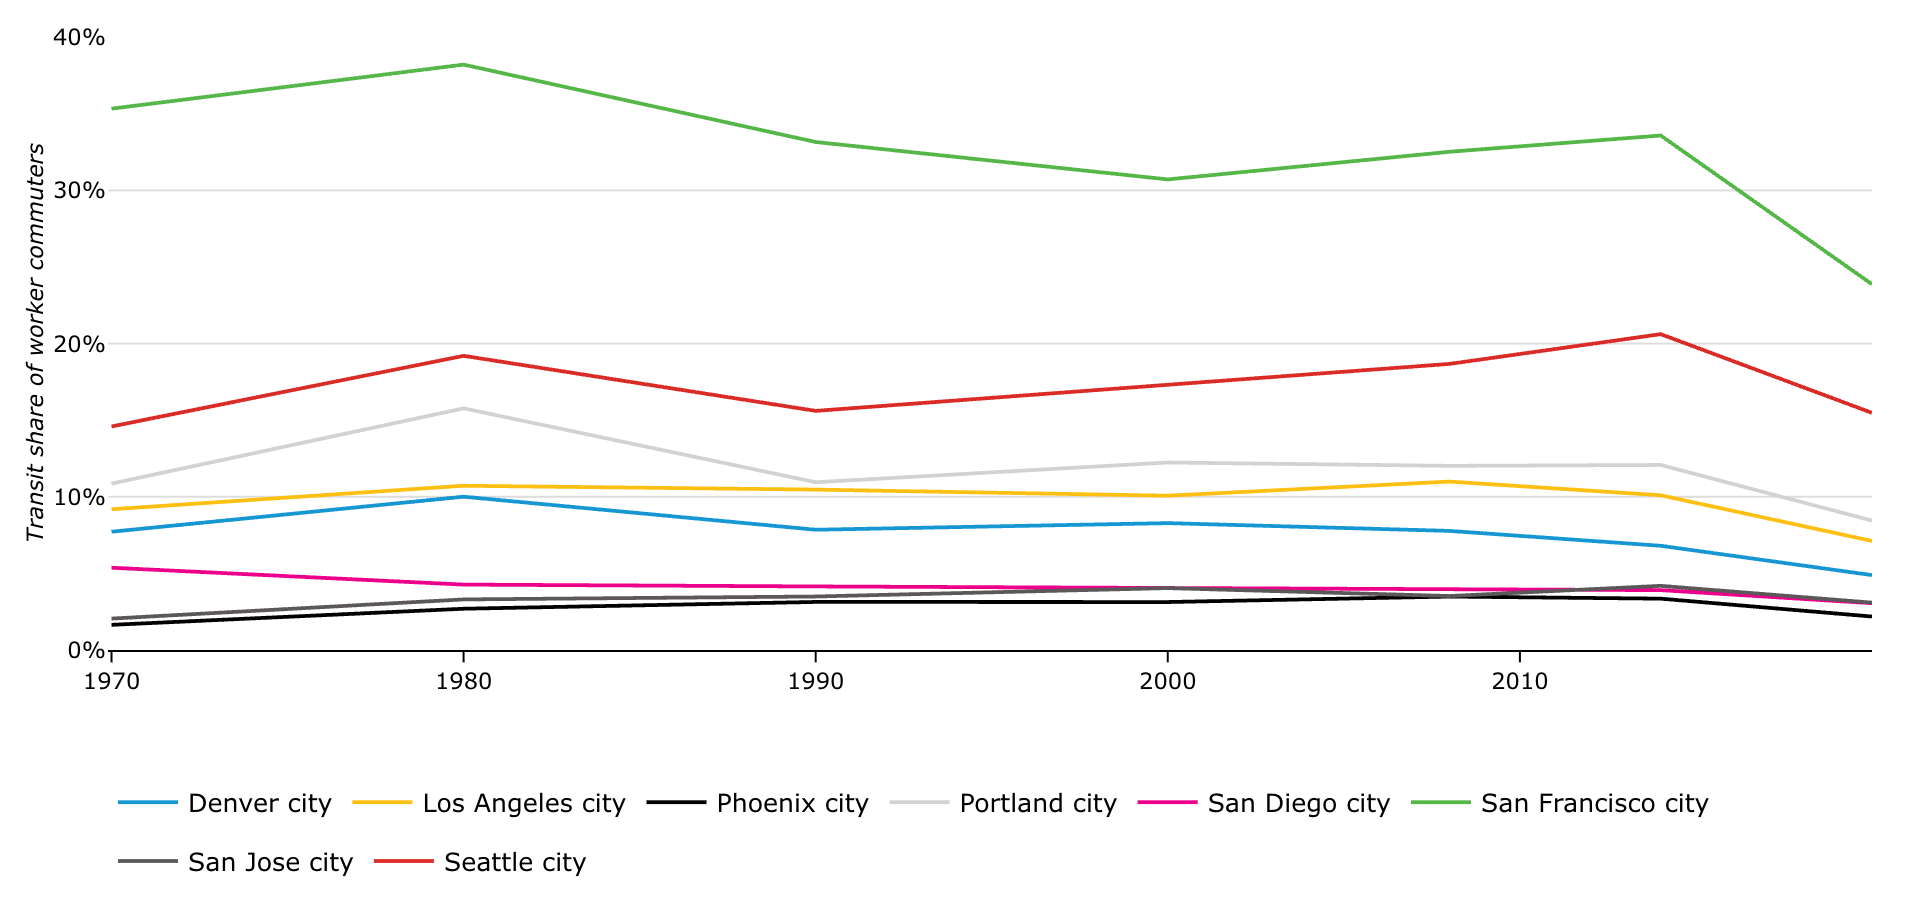
\includegraphics[width=\linewidth]{West.png}
    \\ {\footnotesize West}

\end{columns}

\end{frame}
\begin{frame}{Model Environment}
Consider a metropolitan area with locations $S = \{1,2,\dots,N\}$ partitioned into municipalities $g \in G$.

\vspace{0.35cm}
\begin{itemize}
    \item Each location has fixed land endowment $\bar H_i$.
    \item Land can be allocated between residential and commercial use:
    \[
    H_i^R + H_i^F \leq \bar H_i.
    \]
    \item Zoning restricts feasible development intensity in each location.
    \item Commuting costs depend on transportation infrastructure and congestion\citep{Bordeu2026-df}:
    \[
    \tau_{ijr} = \tau_{ijr}(I^R, I^T, n).
    \]
\end{itemize}

\vspace{0.25cm}
There are three types of agents: households, firms, and governments.
\end{frame}

\begin{frame}{Households and Firms}
\begin{columns}[T]
\column{0.54\textwidth}
\textbf{Households}
\begin{itemize}
    \item Choose residence location $i$
    \item Choose workplace location $j$
    \item Choose commuting route $r \in R_{ij}$
    \item Value wages, rents, amenities, and commuting cost
\end{itemize}

\vspace{0.25cm}
A convenient reduced-form indirect utility is:
\[
V_{ijr}(\omega) \propto \frac{B_i}{\tau_{ijr}} \frac{w_j}{(q_i^R)^{1-\beta}} v_{ijr}(\omega).
\]

\column{0.46\textwidth}
\textbf{Firms}
\begin{itemize}
    \item Produce a tradable good at workplace location $j$
    \item Use labor $L_j$ and commercial land $H_j^F$
\end{itemize}

\[
Y_j = A_j F(L_j, H_j^F).
\]

\vspace{0.2cm}
Competition determines labor demand and commercial land demand.
\end{columns}

\vspace{0.35cm}
Household sorting across space depends on wages, rents, amenities, and infrastructure-induced commuting costs.
\end{frame}

\begin{frame}{Government Structure}
\begin{columns}[T]
\column{0.48\textwidth}
\begin{block}{Municipal governments}
\begin{itemize}
    \item Choose local zoning policies $Z_g$
    \item Act as reduced-form representatives of incumbent residents
    \item Care about local property values, amenities, and congestion/crowding\end{itemize}

 $
W^g
=
\sum_{i\in S^g}
\left[
\omega_1 P_i
+\omega_2 B_i^{\text{loc}}
-\omega_3 N_i
\right],
$
\end{block}

\column{0.48\textwidth}
\begin{block}{Metropolitan authority}
\begin{itemize}
    \item Chooses road and transit investment
    \item Internalizes regional transport benefits
    \item Takes local zoning as given
\end{itemize}
$\max \; W^M(I^R,I^T; Z)-C(I^{R},I^{T}),
$
\end{block}
\end{columns}

\end{frame}

\begin{frame}{Decentralized Equilibrium and Inefficiency}
A decentralized equilibrium features:
\begin{itemize}
    \item optimal household location, workplace, and route choices,
    \item optimal firm labor and commercial land choices,
    \item municipal zoning choices,
    \item metropolitan road and transit investment,
    \item market clearing in residential land, commercial land, and labor.
\end{itemize}

\vspace{0.35cm}
\begin{block}{Source of inefficiency}
Municipalities restrict development of housing to protect incumbent interests, but do not internalize the broader metropolitan costs in housing supply, commuting, and transit effectiveness.
\end{block}


\end{frame}


\begin{frame}{Efficient Benchmark}
\begin{block}{Planner's problem}
A coordinated planner jointly chooses transportation investment and zoning to maximize aggregate metropolitan welfare.
\[
\max_{I^R,I^T,Z}
\; W(I^R,I^T,Z)-C(I^R,I^T),
\]

\end{block}


\vspace{0.35cm}
Comparing the decentralized equilibrium to this benchmark reveals whether fragmented governance leads to excessive sprawl and underutilized transit-oriented development.
\end{frame}


\begin{frame}{Reference}

\printbibliography
    
\end{frame}

\end{document}
